\documentclass{agony}
\usepackage{pgfplots}
\usepgfplotslibrary{fillbetween}
\usetikzlibrary{patterns}

\title{MATH 138 Winter 2021: Practice Assignment 4}

\begin{document}

\begin{prob}
  Determine whether each integral is convergent or divergent.
  If it is convergent, evaluate it.
  If divergent, justify why it is divergent.
\end{prob}
\begin{enumerate}[(a)]
  \item $\int_{-\infty}^\infty(x^3-3x^2) \dd{x}$
        \begin{sol}
          Notice that we can distribute
          $\int_{-\infty}^\infty(x^3-3x^2) \dd{x} = \int_{-\infty}^\infty x^3 \dd{x} - 3\int_{-\infty}^\infty x^2 \dd{x}$.
          Since $x^3$ is odd, the term goes to zero.
          By the $p$-test, the $x^2$ term diverges.
          Therefore, the integral diverges.
        \end{sol}
  \item $\int_0^4 \frac{1}{x^2-x-2} \dd{x}$
        \begin{sol}
          Notice that $x^2 - x - 2 = (x-2)(x+1)$ so there is an asymptote at $x=2$.
          We must find $\int_0^2 \frac{1}{x^2-x-2} \dd{x} + \int_2^4 \frac{1}{x^2-x-2} \dd{x}$.
          By partial fractions:
          \[ \int_0^2 \frac{1/3}{x-2} - \frac{1/3}{x+1} \dd{x} = \lim_{t\to2^-} \qty[\frac13 \ln|x-2| - \frac13 \ln|x+1|]_0^t = -\infty \]
          so the integral diverges.
        \end{sol}
  \item $\int_0^{\pi/2} \frac{\cos x}{\sqrt{\sin x}} \dd{x}$
        \begin{sol}
          Let $u = \sin x$.

          Then, $\int_0^{\pi/2} \frac{\cos x}{\sqrt{\sin x}} \dd{x}
            = \int_0^1 \frac{\dd{u}}{\sqrt{u}}
            = \dlim{t}{0^+} \qty[2\sqrt{u}]_t^1$,
          which converges to 2.
        \end{sol}
  \item $\int_0^5 \frac{1}{\sqrt[3]{5-x}} \dd{x}$
        \begin{sol}
          After substituting, we have $\int_5^0 \frac{\dd x}{\sqrt[3]{x}}
            = \dlim{t}{0^+} [\frac32 x^{2/3}]_5^t$,
          converging to $\frac{3\sqrt[3]{25}}{2}$.
        \end{sol}
  \item $\int_1^\infty \frac{e^{1/x}}{x^2} \dd{x}$
        \begin{sol}
          Notice that if we let $u = e^{1/x}$, then $\dd{u} = -\frac{e^{1/x}}{x^2}$.

          So we have $\dilim{t} \int_1^t -\dd u = \dilim{t} \qty[-e^{1/x}]_1^t
            = - e^0 + e^1 = e - 1$
          which converges.
        \end{sol}
  \item $\int_1^\infty \frac{\ln x}{x^2} \dd{x}$
        \begin{sol}
          Integrate by parts:
          \[
            \int \frac{\ln x}{x^2} \dd{x}
            = -\frac{\ln x}{x} - \int \frac{-\dd x}{x^2}
            = -\frac{1+\ln x}{x} + C
          \]
          Then, $\dilim{t} -\frac{1+\ln x}{x} \big|_1^t = 1$
          converges by the Fundamental Log Limit.
        \end{sol}
  \item $\int_0^1 \frac{e^{1/x}}{x^3} \dd{x}$
        \begin{sol}
          Use the same substitution as (e).
          Then, integrating by parts:
          \[
            \int \frac{e^{1/x}}{x^3} \dd{x}
            = -\frac{e^{1/x}}{x} - \int \frac{e^{1/x}}{x^2} \dd{x}
            = -\frac{e^{1/x}}{x} + e^{1/x}
          \]
          And the limit $\dlim{t}{0^+} \qty[-\frac{e^{1/x}}{x} + e^{1/x}]_t^1
            = \dlim{t}{0^+} \qty[0 + \frac{e^{1/t}}{t} - e^{1/t}] = \infty$
          diverges.
        \end{sol}
\end{enumerate}

\begin{prob}
  Use the Comparison Theorem to determine whether each integral is convergent or divergent.
\end{prob}
\begin{enumerate}[(a)]
  \item $\int_1^\infty \frac{2 + e^{-x}}{x} \dd{x}$
        \begin{prf}
          By the $p$-test, $\int_1^\infty \frac{\dd x}{x}$ diverges.
          But $1+e^{-x}$ is positive, so $\frac{2 + e^{-x}}{x} > \frac{1}{x} > 0$.
          Therefore, by the Comparison Theorem, $\int_1^\infty \frac{2 + e^{-x}}{x} \dd{x}$ diverges.
        \end{prf}
  \item $\int_1^\infty \frac{1 + \sin^2 x}{\sqrt{x}} \dd{x}$
        \begin{prf}
          By the $p$-test, $\int_1^\infty \frac{\dd x}{\sqrt{x}}$ diverges.
          For $x > 1$, $\frac{\sin^2 x}{\sqrt{x}} > 0$, so we have
          $\frac{1 + \sin^2 x}{\sqrt{x}} > \frac{1}{\sqrt{x}} > 0$.
          By the Comparison Theorem,
          $\int_1^\infty \frac{1 + \sin^2 x}{\sqrt{x}} \dd{x}$ must diverge.
        \end{prf}
\end{enumerate}

\begin{prob}
  Consider the following integrals:
\end{prob}
\begin{enumerate}[(a)]
  \item Prove that $\int_e^\infty \frac{\cos x^2}{x^2 \ln x} \dd{x}$ is convergent.
        \begin{prf}
          We apply the Absolute Convergence Theorem.
          Notice that for all $x \geq e$, we have $\ln x > 0$ and
          \[
            0 \leq \abs{\frac{\cos x^2}{x^2 \ln x}}
            \leq \frac{1}{x^2 \ln x}
            \leq \frac{1}{x^2}
          \]
          which, by the $p$-test, is convergent.

          Therefore, by the Absolute Convergence Theorem, the integral converges.
        \end{prf}
  \item Prove that $\int_1^\infty \frac{\sin x}{x} \dd{x}$ is convergent.
\end{enumerate}

\begin{prob}
  Prove that if $f(x)$ is continuous on $[0,\infty)$
  and $\dilim{x} f(x) = \alpha > 0$ (or $\alpha = \infty$),
  then $\int_0^\infty f(x) \dd{x}$ diverges.
\end{prob}
\begin{prf}
  First, consider when $\alpha$ is finite.
  By the definition of the infinite limit, given $\frac\alpha2$,
  there is a $M > 0$ such that when $x \geq M$, $|f(x) - \alpha| < \frac\alpha2$.
  Since $\alpha$ is positive, this implies $f(x) > \frac\alpha2$.
  Now, $\int_M^\infty \frac\alpha2 \dd{x} = \infty$.
  By the Comparision Theorem, the integral diverges.

  If $\alpha = \infty$, there exists a cutoff $N > 0$ such that when $x > N$, $f(x) > 1$.
  The same logic applies, and the integral must diverge.
\end{prf}

\begin{prob}
  Sketch the region enclosed by the given curves and find the area.
\end{prob}
\begin{enumerate}[(a)]
  \item $y = \cos x$, $y = 2-\cos x$, $0 \leq x \leq 2\pi$
        \begin{sol}
          Doodle with \verb|pgfplots|.
          \begin{center}
            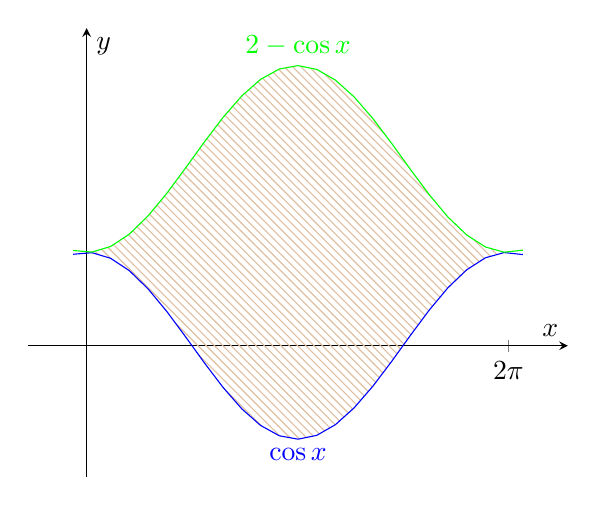
\begin{tikzpicture}
              \begin{axis}[axis lines=middle,
                  xlabel=$x$,
                  ylabel=$y$,
                  enlargelimits,
                  ytick=\empty,
                  xtick={2*pi},
                  xticklabels={$2\pi$}]
                \addplot[name path=F,blue,domain={-.2:6.5}] {cos(deg(x))} node[pos=.5, below]{$\cos x$};
                \addplot[name path=G,green,domain={-.2:6.5}] {2-cos(deg(x))} node[pos=.5, above]{$2-\cos x$};
                \addplot[pattern=north west lines, pattern color=brown!50]fill between[of=F and G, soft clip={domain=0:2*pi}];
              \end{axis}
            \end{tikzpicture}
          \end{center}
          We simply evaluate the integral $\int_0^{2\pi} (2-\cos x) - \cos x \dd{x}$.
          This is $-2\int_0^{2\pi}1 - \cos x\dd{x} = 2[x - \sin x]_0^{2\pi} = 4\pi$.
        \end{sol}
  \item $x = y^4$, $y = \sqrt{2-x}$, $y = 0$
        \begin{sol}
          Doodle, noticing that the POI is $\sqrt[4]{x} = \sqrt{2-x} \iff x = 1$.
          \begin{center}
            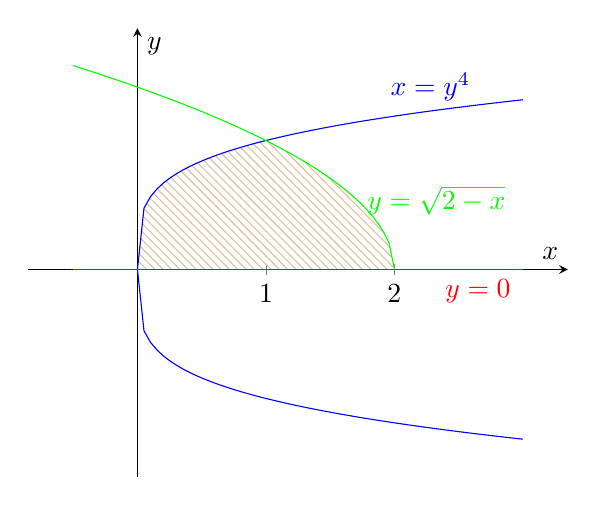
\begin{tikzpicture}
              \begin{axis}[axis lines=middle,
                  xlabel=$x$,
                  ylabel=$y$,
                  enlargelimits,
                  ytick=\empty,
                  xtick={1,2},
                  xticklabels={1,2},
                  samples=60]
                \addplot[name path=F,blue,domain={0:3}] {x^(1/4)} node[pos=.8, above]{$x = y^4$};
                \addplot[blue,domain={0:3}] {-x^(1/4)};
                \addplot[name path=G,green,domain={-.5:2}] {sqrt(2-x)} node[pos=.8, right]{$y = \sqrt{2-x}$};
                \addplot[name path=H,red,domain={-.5:3}] {0} node[pos=.9, below]{$y = 0$};
                \addplot[pattern=north west lines, pattern color=brown!50] fill between [of=F and H, soft clip={domain=0:1}];
                \addplot[pattern=north west lines, pattern color=brown!50] fill between [of=G and H, soft clip={domain=1:2}];
              \end{axis}
            \end{tikzpicture}
          \end{center}
          The two areas are $\int_0^1 \sqrt[4]{x} \dd{x}$ and $\int_1^2 \sqrt{2-x} \dd{x}$.
          The first is $[\frac{4}{5}x^{5/4}]_0^1 = \frac{4}{5}$
          and the second is $\int_0^1 \sqrt{x} \dd{x} = [\frac{2}{3}x^{3/2}]_0^1 = \frac{2}{3}$,
          so the total area is $\frac{22}{15}$.
        \end{sol}
  \item $y = \frac{x^2}{4}$, $y = 2x^2$, $x + y = 3$, $x \geq 0$
        \begin{sol}
          Doodle, noticing that the POI again at $x=1$.
          \begin{center}
            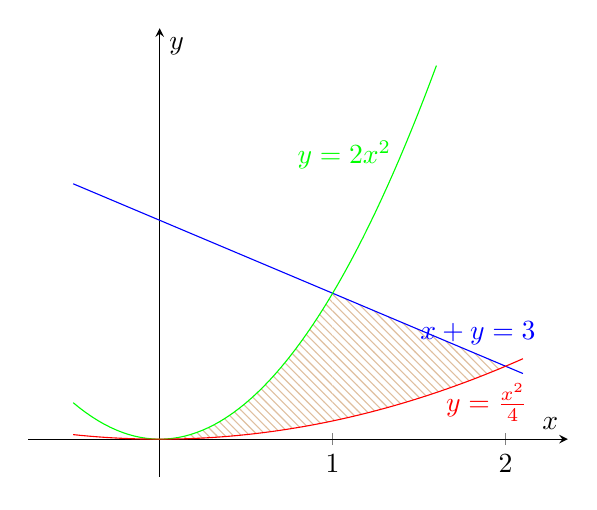
\begin{tikzpicture}
              \begin{axis}[axis lines=middle,
                  xlabel=$x$,
                  ylabel=$y$,
                  enlargelimits,
                  ytick=\empty,
                  xtick={1,2},
                  xticklabels={1,2},
                  samples=60]
                \addplot[name path=F,blue,domain={-.5:2.1}] {3-x} node[pos=.9, above]{$x + y = 3$};
                \addplot[name path=G,green,domain={-.5:1.6}] {2*x^2} node[pos=.8, left]{$y = 2x^2$};
                \addplot[name path=H,red,domain={-.5:2.1}] {x^2/4} node[pos=.9, below]{$y = \frac{x^2}{4}$};
                \addplot[pattern=north west lines, pattern color=brown!50] fill between [of=F and H, soft clip={domain=1:2}];
                \addplot[pattern=north west lines, pattern color=brown!50] fill between [of=G and H, soft clip={domain=0:1}];
              \end{axis}
            \end{tikzpicture}
          \end{center}
          Now, we have $\int_0^1 2x^2 - \frac{x^2}{4} \dd{x} = [\frac23 x^3 - \frac{x^3}{12}]_0^1 = \frac{7}{12}$ for the area between 0 and 1,
          and $\int_1^2 3 - x - \frac{x^2}{4} \dd{x} = [3x - \frac{x^2}{2} - \frac{x^3}{12}]_1^2 = \frac{10}{3} - \frac{29}{12} = \frac{11}{12}$
          for the remainder.

          The sum is $\frac{2}{3}$.
        \end{sol}
\end{enumerate}

\end{document}